
%(BEGIN_QUESTION)
% Copyright 2007, Tony R. Kuphaldt, released under the Creative Commons Attribution License (v 1.0)
% This means you may do almost anything with this work of mine, so long as you give me proper credit

Use Bernoulli's equation to calculate the hydrostatic pressure at the bottom of this water storage tank:

$$\includegraphics[width=15.5cm]{i02987x01.eps}$$

\noindent
{\bf Bernoulli's equation:}

$$z_1 \rho g + {v_1^2 \rho \over 2} + P_1 = z_2 \rho g + {v_2^2 \rho \over 2} + P_2$$

\vskip 10pt

\noindent
Where,

$\rho$ = 1.951 slugs/ft$^{3}$ (for water)

$g$ = 32.2 ft/s$^{2}$

\vskip 10pt

\underbar{file i02987}
%(END_QUESTION)





%(BEGIN_ANSWER)

$P$ = 1373.5 lb/ft$^{2}$ = 9.538 PSI

%(END_ANSWER)





%(BEGIN_NOTES)

%INDEX% Physics, static fluids: Bernoulli's equation applied to hydrostatic head
%INDEX% Physics, static fluids: hydrostatic pressure

%(END_NOTES)


